\section{Robust Large Posynomials} \label{k_term}
Having introduced improved techniques for monomials and two-term posynomials, we now turn to better approximations for posynomial constraints with more than two terms (those associated with $\mathbf{P}$). Two novel methodologies for approximating large posynomials will be presented: the first is only able to transform posynomials whose coefficients are uncertain, while the second can transform posynomials whose coefficients and exponents are uncertain.

\subsection{Linearized Perturbations Formulation} \label{uncertain_coeff}
In the majority of engineering-design constraints, exponents are derived with certainty from physical laws or dimensional analysis, and so programs where uncertainty is only present in the coefficients are common. Let

\begin{displaymath}
\vec{b} = \vec{b}^0 + \textstyle{\sum}_{l=1}^{L}\vec{b}^l\zeta_l
\end{displaymath}
where $\vec{\zeta} \in \mathcal{Z}$ is as given by equation \eqref{perturbation_set}.
The second set of constraints in equation \eqref{categorizedForm} is then equivalent to 

$$
\begin{aligned}
&\max_{\vec{\zeta} \in \mathcal{Z}} \left\{\textstyle{\sum}_{k \in S_{i,j}} e^{\vec{a_{ik}}\vec{x} + b^0_{ik}}e^{\textstyle{\sum}_{l=1}^{L}b^l_{ik}\zeta_l} \right\} &&\leq e^{t_{ij}} &&\forall (i, j) \in \mathbf{P}\\
\Leftrightarrow &\max_{\vec{\zeta} \in \mathcal{Z}} \left\{\textstyle{\sum}_{k \in S_{i,j}}\left(\textstyle{\prod}_{l=1}^{L}e^{b^l_{ik}\zeta_l}\right) e^{\vec{a_{ik}}\vec{x} + b^0_{ik}} \right\} &&\leq e^{t_{ij}} &&\forall (i, j) \in \mathbf{P}\\
\end{aligned}
$$
Thus by applying the following change of variable
$$v_{i,j}^k = e^{\vec{a_{ik}}\vec{x} + b^0_{ik}} \qquad \forall k \in S_{i,j}$$
the constraint above can be rewritten as
\begin{equation}
\max_{\vec{\zeta} \in \mathcal{Z}} \left\{\textstyle{\sum}_{k \in S_{i,j}}\left(\textstyle{\prod}_{l=1}^{L}e^{b^l_{ik}\zeta_l}\right) v_{i,j}^k \right\} \leq e^{t_{ij}} \qquad \forall (i, j) \in \mathbf{P}
\label{linearCon_expPerts}
\end{equation}

Although the constraints in \eqref{linearCon_expPerts} are linear in terms of $\vec{v_{i,j}}$, the perturbations are not affine but exponential, and should be linearized to improve tractability.
 
\subsubsection{Linearizing Perturbations}
The convexity of exponential perturbations (see Figure \ref{perts_convexity}) implies that there exists some half-space $[\vec{f}_{i,j}^k]^T\vec{\zeta} + g_{i,j}^k$ such that 
$$[\vec{f}_{i,j}^k]^T\vec{\zeta} + g_{i,j}^k \geq \textstyle{\prod}_{l=1}^{L}e^{b^l_{ik}\zeta_l} \qquad \forall (i, j) \in \mathbf{P} \qquad \forall k \in S_{i,j}$$
on some finite domain for $\vec{\zeta}$.

\begin{figure}[H]
\captionsetup{justification=centering, font=small}
\begin{center}
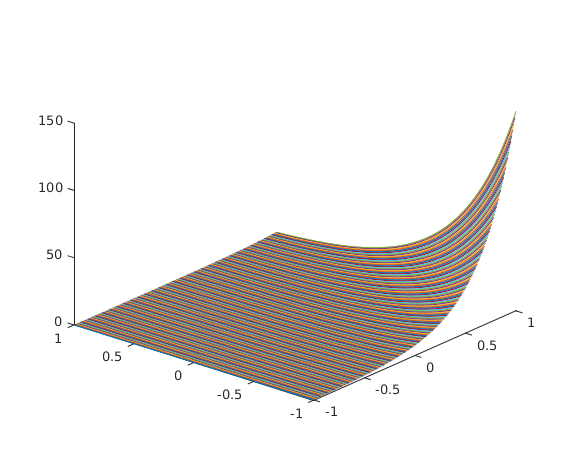
\includegraphics[scale=0.7]{convex.png}
\end{center}
\caption{Example of the convexity of exponential perturbations.}
\label{perts_convexity}
\end{figure}
 
Accordingly, a possible safe approximation of the constraints in equation \eqref{linearCon_expPerts} is
\begin{equation}
\max_{\vec{\zeta} \in \mathcal{Z}} \left\{\textstyle{\sum}_{k \in S_{i,j}}\left([\vec{f}_{i,j}^k]^T\vec{\zeta}\right)v_{i,j}^k \right\} + \textstyle{\sum}_{k \in S_{i,j}}g_{i,j}^k v_{i,j}^k \leq e^{t_{ij}} \qquad \forall (i, j) \in \mathbf{P}
\label{linearCon_linPerts}
\end{equation}

To construct the half-space $[\vec{f}_{i,j}^k]^T\vec{\zeta} + g_{i,j}^k$, and taking into consideration the fact that $-1 \leq \zeta_l \leq 1$ for $l = 1,...,L$, we suggest the following algorithm
\\
\begin{enumerate}
	\item Find the list of vertices $\mathcal{V}$ of the unit box in $\mathbf{R}^L$
	\item Find the list of values $\mathcal{O}$ of $\textstyle{\prod}_{l=1}^{L}e^{b^l_{ik}\zeta_l}$ at the vertices $\mathcal{V}$, note that the $i^{th}$ vertex corresponds to the $i^{th}$ value.
	\item Find the maximum $M_k$ and minimum $m_k$ of $\mathcal{O}$ and their corresponding vertices $\vec{\zeta}_M$ and $\vec{\zeta}_m$.
	\item Solve the least-squares problem 
	$$\min_{\vec{f}_{i,j}^k,\ g_{i,j}^k} \sqrt{\textstyle{\sum}_{\alpha=1}^{|\mathcal{O}|}([\vec{f}_{i,j}^k]^T\mathcal{V}_{\alpha} + g_{i,j}^k - \mathcal{O}_{\alpha})^2}$$
	such that $[\vec{f}_{i,j}^k]^T\vec{\zeta}_M + g_{i,j}^k = M_k$ and $[\vec{f}_{i,j}^k]^T\vec{\zeta}_m + g_{i,j}^k = m_k$
\end{enumerate}
\ \\
Figure \ref{perts_convexity} shows a 2D example where the half-space passes through the highest point (1, -1) and the lowest point (-1, 1).

This half-space is safe for all types of uncertainty sets, although more-specific half-spaces can be constructed for non-exponential uncertainty sets. For instance, with elliptical uncertainty sets, the vertices in the first step might be replaced by an equidistant set of samples from the surface of the uncertainty set.

\subsubsection{Signomial Programming Compatible Constraint}
Equation \eqref{linearCon_linPerts} can be transformed with robust linear programming techniques. Unfortunately, because some components of $\vec{f}_{i,j}^k$ might not be positive, the resulting set of robust constraints is not always GP compatible. Appendix \ref{sigProg} defines signomial programming and clarifies how it is useful to our discussion; in short, it allows the specification and efficient solving of a difference-of-convex program with these negative coefficients.

Signomial problems generally do not need a starting point to solve, but specifying one can speed convergence, and in robust programming there are two quick and obvious candidates for a starting point: the nominal solution of the original program, or the conservative solution of the GP-compatible formulation in \ref{Conservative}.

The number of additional possibly SP constraints needed per uncertain posynomial is equal to the number of uncertain parameters in that posynomial. Decoupling the monomials in each posynomial is equivalent to evaluating the exponential perturbations at its largest value, however, in \eqref{linearCon_linPerts}, the perturbation will be evaluated on a lower point on the half space. As a result, this formulation is guaranteed to be less conservative than that of Section \ref{Conservative}, or the same if both are exact.

\subsection{Best Pairs Formulation}\label{uncertain_exps}
We now discuss a framework for robustifying constraints with uncertain coefficients and exponents. Consider the constraints in $\mathbf{P}$
\begin{equation}
\max_{\vec{\zeta} \in \mathcal{Z}} \left\{\textstyle{\sum}_{k \in S_{i,j}} e^{\vec{a_{ik}}\left(\zeta\right)\vec{x} + b_{ik}\left(\zeta\right)} \right\} \leq e^{t_{ij}} \qquad \forall (i, j) \in \mathbf{P}
\label{second_set}
\end{equation}
Let $\mathcal{P}_{i,j}$ be the set of permutations on $S_{i,j}$, and let $\phi_k$ be the image of an element $k \in S_{i,j}$ under the permutation $\phi \in \mathcal{P}_{i,j}$. Accordingly, \eqref{second_set} is equivalent to  
\begin{equation}
\max_{\vec{\zeta} \in \mathcal{Z}} \left\{\textstyle{\sum}_{k \in S_{i,j}} e^{\vec{a_{i\phi_k}}\left(\zeta\right)\vec{x} + b_{i\phi_k}\left(\zeta\right)} \right\} \leq e^{t_{ij}} \qquad \forall (i, j) \in \mathbf{P} \qquad \phi \in \mathcal{P}_{i,j}
\label{permutation_k_term}
\end{equation}

Our goal is to maximize pairs of monomials while trying to choose the least conservative combination. Let 
$$
\vec{a_{iS_{i,j}^k}}\left(\zeta\right)\vec{x} + b_{iS_{i,j}^k}\left(\zeta\right) = \mathcal{L}^k_{i,j}\quad \forall (i,j) \in \mathbf{P}
$$
where $S_{i,j}^k$ is the $k^{th}$ element of $S_{i,j}$, and assume that $|S_{i,j}|$ is even, such that
$$
\max_{\vec{\zeta} \in \mathcal{Z}} \left\{\textstyle{\sum}_{k=1}^{|S_{i,j}|} e^{\mathcal{L}^{\phi_k}_{i,j}}\right\} \leq \textstyle{\sum}_{k=1}^{|S_{i,j}|/2} \max_{\vec{\zeta} \in \mathcal{Z}} \left\{e^{\mathcal{L}^{\phi_{2k-1}}_{i,j}} + e^{\mathcal{L}^{\phi_{2k}}_{i,j}}\right\}
$$
for any permutation $\phi \in \mathcal{P}_{i,j}$. Therefore
$$
\max_{\vec{\zeta} \in \mathcal{Z}} \left\{\textstyle{\sum}_{k=1}^{|S_{i,j}|} e^{\mathcal{L}^{\phi_k}_{i,j}}\right\} \leq \min_{\phi \in \mathcal{P}_{i,j}}\left\{\textstyle{\sum}_{k=1}^{|S_{i,j}|/2} \max_{\vec{\zeta} \in \mathcal{Z}} \left\{e^{\mathcal{L}^{\phi_{2k-1}}_{i,j}} + e^{\mathcal{L}^{\phi_{2k}}_{i,j}}\right\}\right\}
$$
and
\begin{equation}
\min_{\phi \in \mathcal{P}_{i,j}}\left\{\textstyle{\sum}_{k=1}^{|S_{i,j}|/2} \max_{\vec{\zeta} \in \mathcal{Z}} \left\{e^{\mathcal{L}^{\phi_{2k-1}}_{i,j}} + e^{\mathcal{L}^{\phi_{2k}}_{i,j}}\right\}\right\} \leq e^{t_{ij}} \qquad \forall (i, j) \in \mathbf{P}
\label{min_safe_app}
\end{equation}
is a safe approximation of \eqref{permutation_k_term}. From the fact that
$$
\max(a + b) + \max(c + d) = \max(c + d) +  \max(a + b) = \max(b + a) + \max(d + c)
$$
we see that some perturbations result in identical safe approximations. The permutation set can be modified to contain differing permutations only; let $\mathcal{P}_{i,j}$ represent the set of differing permutations. The number of differing permutations is given by
\begin{equation}
|\mathcal{P}_{i,j}| = \frac{\binom{|S_{i,j}|}{2}\binom{|S_{i,j}|-2}{2}\binom{|S_{i,j}|-4}{2}...\binom{4}{2}}{(|S_{i,j}|/2)!}
\label{no_pert_even}
\end{equation}
If the number of monomial terms for a given posynomial is large, then $|\mathcal{P}_{i,j}|$ might become quite large. Therefore, we might choose to work with a subset $\hat{\mathcal{P}}_{i,j}$ of $\mathcal{P}_{i,j}$, where the permutations are either chosen depending on the structure of the posynomial or randomly selected. Constraints associated with $\mathbf{P}$ will be replaced by 
\begin{equation}
\textstyle{\sum}_{k=1}^{|S_{i,j}|/2} {\displaystyle \max_{\vec{\zeta} \in \mathcal{Z}}} \left\{e^{\mathcal{L}^{\phi_{2k-1}}_{i,j}} + e^{\mathcal{L}^{\phi_{2k}}_{i,j}}\right\}\leq e^{t_{ij}} \qquad \forall (i, j) \in \mathbf{P} \qquad \phi \in \hat{\mathcal{P}}_{i,j}
\label{two_term_max_even}
\end{equation}
The constraints in \eqref{two_term_max_even} are safe approximations for those in \eqref{permutation_k_term}, and equivalent to
\begin{equation}
\begin{aligned}
&\textstyle{\sum}_{k=1}^{|S_{i,j}|/2} e^{z_{ij}^k} &&\leq e^{t_{ij}} \qquad &&\forall (i, j) \in \mathbf{P}\\
&\max_{\vec{\zeta} \in \mathcal{Z}} \left\{e^{\mathcal{L}^{\phi_{2k-1}}_{i,j}} + e^{\mathcal{L}^{\phi_{2k}}_{i,j}}\right\} &&\leq e^{z_{ij}^k} &&\forall (i, j) \in \mathbf{P} \qquad \forall k \in \left\{1,..,|S_{i,j}|/2\right\}
\end{aligned}
\label{two_term_even}
\end{equation}
Accordingly, the robust counterparts in section \ref{RGP} will be safely approximated by
\begin{equation}
\begin{aligned}
&\min &&f_0(x)\\
&\text{s.t.} &&\textstyle{\sum}_{j=1}^{N_e^i} e^{t_{ij}} &&\leq 1 \quad &&\forall i \in 1,..,m\\
& &&\max_{\vec{\zeta} \in \mathcal{Z}} \left\{e^{\mathcal{L}_{i,j}^1} \right\} &&\leq e^{t_{ij}} &&\forall (i,j) \in \mathbf{M}\\
& &&\max_{\vec{\zeta} \in \mathcal{Z}} \left\{e^{\mathcal{L}_{i,j}^1} + e^{\mathcal{L}_{i,j}^2} \right\} &&\leq e^{t_{ij}} &&\forall (i,j) \in \mathbf{N}\\
& &&\textstyle{\sum}_{k=1}^{|S_{i,j}|/2} e^{z_{ij}^k} &&\leq e^{t_{ij}} \quad &&\forall (i,j) \in \mathbf{P}\\
& &&\max_{\zeta \in \mathcal{Z}} \left\{e^{\mathcal{L}^{\phi_{2k-1}}_{i,j}} + e^{\mathcal{L}^{\phi_{2k}}_{i,j}}\right\} &&\leq e^{z_{ij}^k} &&\forall (i,j) \in \mathbf{P}\\
& && && &&\forall k \in \left\{1,..,|S_{i,j}|/2\right\}\\
& && && && \phi \in \hat{\mathcal{P}}_{i,j}\\
\end{aligned}
\label{GP_counterparts_tractable}
\end{equation}

Each constraint in \eqref{GP_counterparts_tractable} is composed of monomials, two-term posynomials, or data-deprived large posynomials, and so the program is tractable.

Our final step is finding good permutations, i.e. permutations that will make our solution less conservative. For that sake, the following lemma will be utilized

\begin{lemma}
Considering the two optimization problems 
$$
\begin{aligned}
&\min f(\vec{x})\\
&\text{s.t. } \mathcal{S}_i(\vec{x}) \leq 0 \qquad i = 1,2,...,n
\end{aligned}
$$
and
$$
\begin{aligned}
&\min f(\vec{x})\\
&\text{s.t. } \mathcal{T}_i(\vec{x}) \leq 0 \qquad i = 1,2,...,n
\end{aligned}
$$
let $\vec{x}_1$ and $\vec{x}_2$ be their respective solutions. If $\mathcal{T}_i(\vec{x}_1) \leq \mathcal{S}_i(\vec{x}_1) \ \ \forall i \in \left\{1,2,...,n\right\}$, then $f(\vec{x}_2) \leq f(\vec{x}_1)$
\label{the_lemma}
\end{lemma}
\begin{proof}
$$\mathcal{T}_i(\vec{x}_1) \leq \mathcal{S}_i(\vec{x}_1) \leq 0 \quad \forall i \in \left\{1,2,...,n\right\} $$ 
So $\vec{x}_1$ is a feasible solution for the second optimization problem. But since $\vec{x}_2$ is the optimal solution of the second problem, then
$$f(\vec{x}_2) \leq f(\vec{x}_{feasible}) \implies f(\vec{x}_2) \leq f(\vec{x}_1)$$
\ 
\end{proof}

Starting from the above lemma, the algorithm below illustrates how relatively good permutations might be chosen:
\\
\begin{enumerate}
\item Randomly choose the permutations $\phi$ from the set $\hat{\mathcal{P}}_{i,j}$ $\forall (i,j) \in \mathbf{P}$
\item Solve the optimization problem in \eqref{GP_counterparts_tractable}, and let $\vec{x}_1$ be the solution
\item Repeat
\begin{enumerate}
\item $\forall (i,j) \in \mathbf{P}$, select the new permutations $\phi \in \hat{\mathcal{P}}_{i,j}$ such that $\phi$ minimizes $\textstyle{\sum}_{k=1}^{|S_{i,j}|/2} {\displaystyle \max_{\vec{\zeta} \in \mathcal{Z}}} \left\{e^{\mathcal{L}^{\phi_{2k-1}}_{i,j}} + e^{\mathcal{L}^{\phi_{2k}}_{i,j}}\right\}\bigg\rvert_{\vec{x}_i}$
\item Solve the optimization problem in \eqref{GP_counterparts_tractable}, and let $\vec{x}_i$ be the solution
\item If $\vec{x}_i = \vec{x}_{i-1}$ : break
\end{enumerate}
\end{enumerate}
\ \\
Although the final solution might not be the globally least-conservative over all possible permutations it is guaranteed to be the locally least-conservative given the descent algorithm based on Lemma \eqref{the_lemma}. The Best Pairs Formulation is guaranteed to be less-conservative than the Two-term formulation because it involves less monomial decoupling and fewer piecewise-linear approximations.